\setcounter{page}{1}

\section{Ziel}
Ziel des Versuches ist die Bestimmung der magnetischen Felder verschiedener Spulenandordnungen.

\section{Theorie}

Bewegte Ladungen erzeugen magnetische Felder, welche durch die magnetische Feldstärke $\vec{H}$ beschrieben werden.
Unter der Vorraussetzung, dass die magnetischen Momente der Atome eines Körpers durch die Wärmebewegung
statistisch verteilt sind, lässt sich folgender Zusammenhang zwischen
magnetischer Flussdichte $\vec{B}$ und magnetischer Feldstärke $\vec{H}$ aufstellen:
\begin{equation}
  \vec{B}=\mu \cdot \vec{H}=\mu_0 \mu_r \cdot \vec{H} \label{eqn:mFdus} .
\end{equation}
Dabei ist $\mu_0$ = \SI{4\pi e-7}{\newton\per\ampere\squared} die Vakuumpermeabilität und $\mu_r$ die relative Permeabilität.
Die magnetische Flussdichte lässt sich bei stromdurchflossenden Leitern durch das Biot-Savart-Gesetz
\begin{equation}
  d\vec{B} = \frac{\mu_0 I}{4 \pi} \frac{d\vec{s} \times \vec{r}}{r^3} \label{eqn:bs}
\end{equation}
bestimmen, wobei $I$ hier die Stromstärke ist.
Für eine Spule mit $n$ Windungen gilt somit:
\begin{equation}
  \vec{B}(x) =n \cdot \frac{\mu_0 I}{2} \frac{R^2}{(R^2 + x^2)^{\frac{3}{2}}} \vec{e_x} \label{eqn:Spule}.
\end{equation}
Dabei ist $R$ der Spulenradius und $x$ der Abstand zum Spulenzentrum.
Handelt es sich bei der Spule um einen Solenoiden, also eine langestreckte Spule,
so ist die magnetische Feldstärke $\vec{H}$ in der Mitte der Spule konstant.
Ebenso verlaufen die Feldlinien parallel zur Spulenachse und das magnetische Feld ist homogen.
Außerhalb der Spule gilt dies jedoch nicht, da sich die Feldlinien dort auffächern.
Für den Fall $l \gg d$, wobei $l$ die Länge und $d$ der Durchmesser ist,
gilt für die homogene magnetische Flussdichte $\vec{B}$:
\begin{equation}
  \lvert \vec{B} \rvert= \mu \frac{n}{l}I \label{eqn:Solenoid}.
\end{equation}
Wird nun ein Solenoid zu einem Torus mit Radius $r_T \ll l$ umgeformt,
so ist keine äußere magnetische Flussdichte mehr vorhanden.
Innerhalb des Toroids lässt sich die magnetische Flussdichte $\vec{B}$ mit $l=2 \pi r_T$ analog zu \eqref{eqn:Solenoid}
bestimmen:
\begin{equation}
  \lvert \vec{B} \rvert= \mu \frac{n}{2 \pi r_T}I .
\end{equation}

Um ein homogenes Magnetfeld zu erzeugen, kann auch ein Helmholtz-Spulenpaar eingesetzt werden,
welches aus zwei gleichsinnig vom Strom $I$ durchflossenen Kreisspulen besteht.
Diese werden so positioniert, dass ihre Achsen zusammenfallen.
Aufgrund des Superpositionsprinzips folgt aus Gleichung \eqref{eqn:Spule} die Gleichung
  \begin{equation}
    \lvert \vec{B} \rvert = n\cdot \frac{\mu_0 I R^2}{(R^2 + x^2)^{\frac{3}{2}}} ,
    \label{eqn:bfeld}
  \end{equation}
wobei $d = 2x$ gilt.
$d$ ist dabei der Abstand der beiden Spulen.
Befindet sich ein ferromagnetischer Stoff in einer Spule, so steigt der Betrag der magnetischen Flussdichte $\vec{B}$ und
es gilt
\begin{equation}
  \vec{B}=\mu_0 \left(\vec{H}+\vec{M} \right) , \label{eqn:kbmirwasauszudenken}
\end{equation}
wobei mögliche Randeffekte mit $\vec{H}=\vec{H}_0 + \vec{H}_R$ berücksichtigt werden und $\vec{M}$ durch die
Erhöhung der Feldstärke $\vec{B}_\text{Fe}=\mu_0 \vec{M}$ gegeben ist.

\begin{wrapfigure}{r}{0.4\textwidth}
  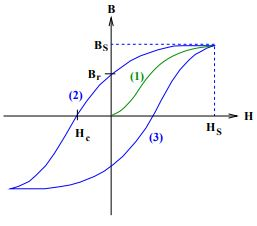
\includegraphics{Text/Bilder/Kurvenverlauf.jpg}
  \caption{Hysteresekurve\cite[3]{sample}}
  \label{figure:HK}
\end{wrapfigure}

Ursache für den höheren Betrag der magnetischen Flussdichte $\vec{B}$ sind die Weiß'schen Bezirke innerhalb des Materials.
In solchen sind magnetische Momente vorhanden, die sich, auch ohne äußeren Einfluss, parallel zueinander ausrichten, weshalb
ferromagnetische Stoffe ein permanentes magnetisches Moment aufweisen.
Wirkt jedoch ein äußeres magnetisches Feld auf einen ferromagnetischen Stoff ein, richten sich die magnetischen Momente
in den einzlenen Weiß'schen Bezirken solange aus,
bis alle magnetischen Momente mit der Ausrichtung des äußeren Feldes übereinstimmen.
Da der Ausgangszustand jedoch nicht wieder durch Abwesenheit des magnetischen Feldes erreicht wird, bleibt Restmagnetismus
zurückt.
Dieses Phänomen wird durch die Hysteresekurve (s. Abbildung \ref{figure:HK}) beschrieben.
Die hier dargestellte Kurve ist jedoch nicht allgemeingültig,
sondern dient nur zur groben Darstellung, da der genaue Verlauf von der Vorgeschichte des Materials abhängt.

Wie in Abbildung \ref{figure:HK} zu sehen, bleibt, wie bereits erwähnt, Restmagnetisierung zurück, wenn kein äußeres magnetisches
Feld anliegt. Dies wird als Remanenz bezeichnet.
Als Koerzitätskraft $H_C$ wird die Feldstärke bezeichnet, bei dem die Restmagnetisierung aufgehoben wird.
Der Wert $B_S$ wird als Sättigungswert bezeichnet.
\\
Da die relative Permeabilität bei ferromagnetischen Stoffen Größenordnungen von $10^2$ bis $10^7$ annehmen kann, verliert die
Gleichung \eqref{eqn:mFdus} ihre Gültigkeit und Gleichung \eqref{eqn:kbmirwasauszudenken} kann zu
\begin{equation}
  \vec{B} \approx \mu_0 \vec{M}
\end{equation}
umgeschrieben werden.
